\cleardoublepage
\chapter{DOKUMENTASI KOORDINASI TEKNIS (WAWANCARA 2)}
\label{chap:lampiran_b}

\section{Dokumentasi Foto Wawancara 2}
Berikut adalah dokumentasi visual pada saat koordinasi teknis dengan pihak pengelola gedung mengenai pengadaan dan instalasi perangkat keras.

\begin{figure}[htbp]
    \centering
    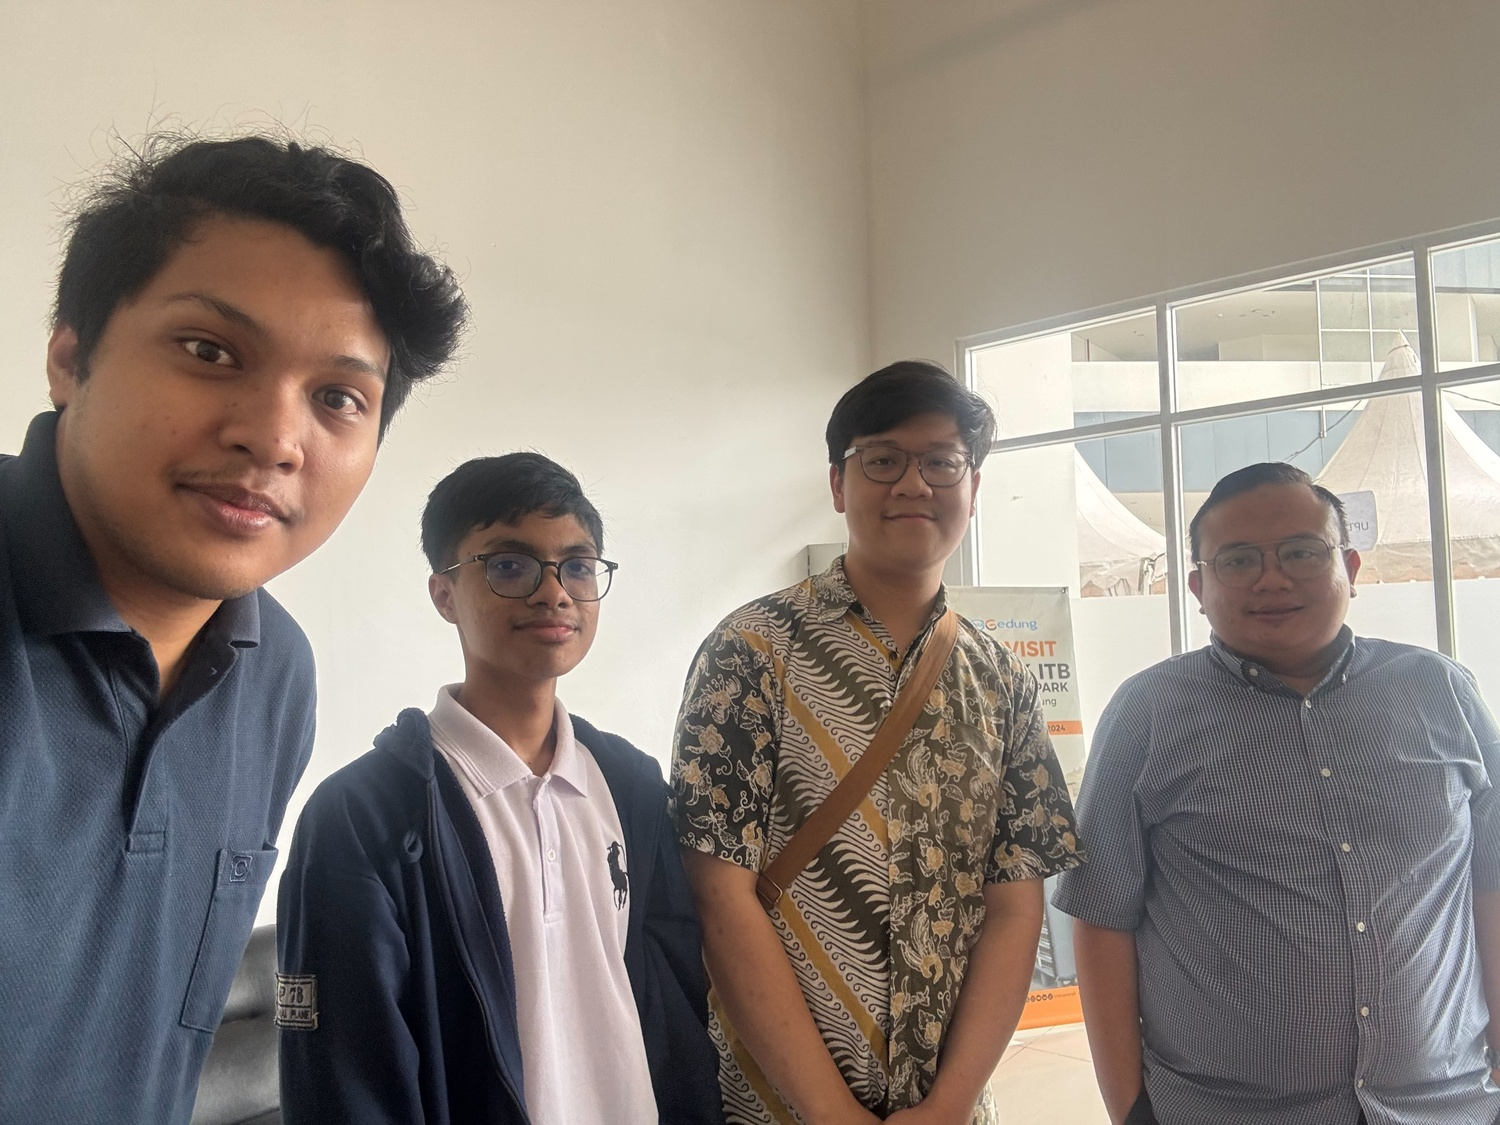
\includegraphics[width=0.6\textwidth]{images/wawancara2_1.png}
    \caption{Dokumentasi Pelaksanaan Wawancara 2 (B)}
\end{figure}

\section{Transkrip Wawancara 2}
Wawancara kedua dilakukan untuk membahas aspek teknis instalasi, persyaratan administratif pengadaan vendor, serta spesifikasi integrasi sistem dengan infrastruktur ITB. Berikut adalah transkrip lengkap dari diskusi tersebut:

\begin{longtable}{|c|p{0.35\textwidth}|p{0.55\textwidth}|}
\hline
\textbf{No} & \textbf{Pewawancara (Mahasiswa)} & \textbf{Narasumber (Pengelola Gedung)} \\ \hline
\endfirsthead
\hline
\textbf{No} & \textbf{Pewawancara (Mahasiswa)} & \textbf{Narasumber (Pengelola Gedung)} \\ \hline
\endhead
\hline
\endfoot
\hline
\endlastfoot
1 & Bagaimana status pengadaan atau pergerakan vendor untuk pemasangan gerbang (\textit{gate}) di lobi saat ini? & Kami sudah mulai survei dan ada lima vendor yang akan diikutsertakan tender. Kalau tim mahasiswa punya penawaran (sistem dan alat), buat saja surat proposal agar pimpinan DKST yang memutuskan. \\ \hline
2 & Terkait instalasi perangkat kerasnya nanti, bagaimana teknis pelaksanaannya di lapangan? & Tinggal menarik kabel LAN, kabel kontrol (AWG), dan kabel power. Nanti tinggal dilakukan proses \textit{coring} lantai untuk menyambungkan kabel langsung ke server kami di lantai B1. \\ \hline
3 & Apakah diperlukan surat resmi untuk proses implementasi dan pemasangan ini? & Iya, harus ada surat resmi dari dosen pembimbing yang ditujukan kepada pimpinan DKST. Harus ada dokumentasi hitam di atas putih untuk setiap pekerjaan fisik atau penelitian di gedung, tidak bisa hanya lisan. \\ \hline
4 & Apakah ada spesifikasi teknis khusus atau \textit{requirement} dari ITB untuk perangkat akses ini? & Perangkat wajib mendukung koneksi TCP/IP, PoE, \textit{interface} standar Wiegand (W26/W34), dan RS485. Frekuensi RFID di 13,56 MHz. Vendor/Sistem juga harus menyediakan API/SDK, mampu sinkronisasi data pegawai dari HRIS ITB, mendukung \textit{centralized management}, serta menjamin keamanan komunikasi via HTTPS/SSL. \\ \hline
5 & Untuk perangkat \textit{gate} fisiknya, apakah diserahkan kepada kami atau ada kriteria khusus? & Dibebaskan, silakan \textit{improve}. Yang penting akurasi deteksinya mendekati 80\%-90\% dan datanya \textit{match} saat registrasi. Untuk fisik \textit{gate}-nya pimpinan menyarankan model \textit{swing} atau \textit{flap barrier}. \\ \hline
6 & Untuk operasional tamu reguler, bagaimana ekspektasi alurnya? & Tamu reguler mendaftar ke lobi, menukar KTP, dan diberikan kartu RFID. Pengenalan wajah (\textit{face recognition}) khusus karyawan. Jika ada tamu VIP/jangka panjang, baru kita daftarkan ke sistem wajahnya. \\ \hline
7 & Tadi Bapak sempat menyinggung soal akses lift, bagaimana integrasinya? & Setelah personel melewati gerbang lobi dan masuk ke lift, mereka tidak bisa menekan tombol lantai tujuan kecuali menggunakan kartu akses yang sesuai dengan otoritas lantai masing-masing. \\ \hline
8 & Bagaimana dengan model bisnis dan status kepemilikan alat setelah implementasi tugas akhir ini selesai? & Kalian harus diskusikan dan pastikan dulu dengan dosen pembimbing kontraknya seperti apa. Apakah ini hibah (gratis), sewa, atau jual putus (B2B) di mana kalian bertindak sebagai vendor. Ini harus jelas di awal karena infrastruktur fisik (seperti \textit{coring} lantai dan kabel) membutuhkan biaya yang tidak sedikit. Saya bagian teknis lapangan, urusan bisnis nanti dengan pimpinan DKST. \\ \hline
\end{longtable}
